% Template for a Computer Science Tripos Part II project dissertation
\documentclass[12pt,a4paper,twoside,openright]{report}
\usepackage[pdfborder={0 0 0}]{hyperref}    % turns references into hyperlinks
\usepackage[margin=25mm]{geometry}  % adjusts page layout
\usepackage{graphicx}  % allows inclusion of PDF, PNG and JPG images
\usepackage{verbatim}
\usepackage{pdfpages} % allows inclusion of non tex project proposal
\usepackage{docmute}   % only needed to allow inclusion of proposal.tex

\raggedbottom                           % try to avoid widows and orphans
\sloppy
\clubpenalty1000%
\widowpenalty1000%

\renewcommand{\baselinestretch}{1.1}    % adjust line spacing to make
                                        % more readable
\begin{document}

\bibliographystyle{plain}


%%%%%%%%%%%%%%%%%%%%%%%%%%%%%%%%%%%%%%%%%%%%%%%%%%%%%%%%%%%%%%%%%%%%%%%%
% Title


\pagestyle{empty}

\rightline{\LARGE \textbf{Oliver Black}}

\addcontentsline{toc}{chapter}{Cover Sheet}

\vspace*{60mm}
\begin{center}
\Huge
\textbf{Software IPv6 Router in Rust} \\[5mm]
Computer Science Tripos -- Part II \\[5mm]
Selwyn College \\[5mm]
\today  % today's date
\end{center}

\newpage
\addcontentsline{toc}{chapter}{Declaration of Originality}
\section*{Declaration of Originality}

I, Oliver Black of Selwyn College, being a candidate for Part II of 
the Computer Science Tripos, hereby declare
that this dissertation and the work described in it are my own work,
unaided except as may be specified below, and that the dissertation
does not contain material that has already been used to any substantial
extent for a comparable purpose.

\bigskip
\leftline{Signed Oliver Black}

\medskip
\leftline{Date \today}

%%%%%%%%%%%%%%%%%%%%%%%%%%%%%%%%%%%%%%%%%%%%%%%%%%%%%%%%%%%%%%%%%%%%%%%%%%%%%%
% Proforma, table of contents and list of figures

\pagestyle{plain}

\chapter*{Proforma}
\addcontentsline{toc}{chapter}{Proforma}

{\large
\begin{tabular}{ll}
Name:               & \bf Oliver Black                      \\
College:            & \bf Selwyn College                     \\
Project Title:      & \bf Software IPv6 Router in Rust \\
Examination:        & \bf Computer Science Tripos -- Part II, July 2001  \\
Word Count:         & \bf "FIX ME\& footnote" \footnotemark[1]
                       \\
Project Originator: & Oliver Black \& Dr Richard Watts      \\
Supervisor:         & Andrew Moore                   \\ 
\end{tabular}
}
\footnotetext[1]{This word count was computed
by \texttt{detex diss.tex | tr -cd '0-9A-Za-z $\tt\backslash$n' | wc -w}
}
\stepcounter{footnote}


\section*{Original Aims of the Project}

The IPv6 standard contains a large number of complex requirements, complicating understanding. I aim to design and implement a simple IPv6 router using Rust\cite{rust} that behaves as specified in the IPv6 RFCs\cite{ipv6_rfc}. This router should implement the minimum functionality required by the relevant standards, yet still be functional, minimal, \& stable.  Rust is a new programming language that aims to be as fast as C while maintaining memory safety, I wanted to understand how practical it was to develop in.

\section*{Work Completed}

Despite having initial difficulties setting up my test environment using Mininet\cite{mininet}, due to its lack of support for IPv6, I successfully implemented a functioning IPv6 router in rust that met almost all of my core requirements. Both the router itself, and the test bench, are available for public use.  TODO mention speedup/code coverage/size/RFC coverage/throughput AND fill rest in when main body done. mention how ambitious original claims were

\section*{Special Difficulties}

None. TODO fill in

\tableofcontents
\addcontentsline{toc}{chapter}{Table of Contents}
\listoffigures
\addcontentsline{toc}{chapter}{List of Figures}

\newpage
\section*{Acknowledgements}

Many thanks to:
\begin{itemize}
\item My supervisor Andrew Moore for his helpful advice.
\item My Director of Studies Dr Richard Watts for his guidance.
\item Friends \& family for proofreading.
\end{itemize}

%%%%%%%%%%%%%%%%%%%%%%%%%%%%%%%%%%%%%%%%%%%%%%%%%%%%%%%%%%%%%%%%%%%%%%%
% now for the chapters

\pagestyle{headings}

\chapter{Introduction}
Slowly but surely the internet is making progress towards IPv6, and how do pages of Requests for Comments (RFCs) translate into real world network components. The aim of this project was to develop an IPv6 Router in Rust that explores the functionality of IPv6, and how different parts of the various standards fit together. The project has been a success, I have produced a functioning router and accompanying test suite.

\bigskip

Due to the popularity of the Internet, there are now not enough IPv4 addresses to go around. IPv6 is the incoming internet addressing standard that solves numerous issues with IPv4.  Primarily it increases the number of addresses, however it also fixes many flaws in the IPv4 design, and standardises common non-standard practices. For example, the Time To Live in IPv4 was defined partly in terms of seconds left to live\cite{ipv4_rfc}, but in practice was decremented by 1 every hop between nodes. In IPv6 the field is accurately renamed to Hop Limit, and is now defined in terms of hops between nodes (as opposed to seconds). Many subtle decisions like this have gone into the IPv6 standard, with an aim to making an internet that works well, rather than one that just works.

\bigskip

Rust\cite{rust} is an up and coming modern low level programming language. It aims to match the performance of C++ without sacrificing memory safety, and avoiding garbage collection. It does this through zero-cost high level abstractions such as \textit{ownership} and \textit{lifetimes}. For example, if you pass a struct to a function, that function then owns that struct, with it being inaccessible after the function returns. It is possible for functions to borrow values instead, using "\texttt{\&}", similar to passing by reference.  I chose Rust for my project as it can be easier to debug than C or C++, but mainly because I was interesting in learning Rust.

\bigskip

Mininet\cite{mininet} is an open source virtual network simulator that was developed at Stanford and until 2016 was used in the Part 1B Computer Networking course, it is written in Python.  It creates lightweight virtual networks by making use of Linux's \textit{networked namespaces}, allowing processes to share a kernel, yet be behind different network interfaces. This made it the ideal candidate to build my router and test suite on top of.

\bigskip

Routers are the backbone of the internet, at the most simple level many of them have a \textit{control plane} that deals with addressing, and a \textit{forwarding plane} that deals with actually sending packets. There are many open source routers out there, but almost all of them have lots of IPv4 code. This makes it difficult to isolate and understand how the IPv6 part actually works.  Starting from scratch allows you to avoid having to deal with IPv4 at all.  Using the IPv6 standard as a framework, combined with some knowledge about the internals of routers, it is possible to develop and IPv6 router that is stable, small, simple, \& fast.

\chapter{Preparation}

Before starting the implementation lots of research and design needed to be done. Lots of research was done into IPv6 RFCs and which aspects were required to be implemented, and which were not. The router software was then designed to provide a framework within which these aspects could be implemented.  Additionally a test plan needed to be made, to enable effective evaluation of the finished product.

\section{Research}
An analogous project for IPv4 called Simple Router already exists\cite{simple_router} (it used to be a recommended extension task for the Part 1B Computer Networking course).  It is implemented in C, but it ran on top of Mininet.  The implementation didn't help at all (due to being in C and for IPv4), but it running on Mininet demonstrates that running a router on Mininet is feasible.  Additionally the Mininet code that ran the Simple Router helped me in designing my test bench.

\bigskip

Most of my research time however was spent reading RFCs related to IPv6.  The main RFC\cite{ipv6_rfc} specifies everything you need to know about IPv6 packets. This describes the contents of the main IPv6 header, \hyperref[fig::ipv6_header]{Figure }\ref{fig::ipv6_header}, including how the fields (e.g. \textit{Hop Limit}) are modified for packets in transit. Additionally this includes the extension headers that need to be implemented by a router, when the packet in question is not addressed to the router this turns out to be none. 

\begin{figure}
\begin{verbatim}
+-+-+-+-+-+-+-+-+-+-+-+-+-+-+-+-+-+-+-+-+-+-+-+-+-+-+-+-+-+-+-+-+
|Version| Traffic Class |           Flow Label                  |
+-+-+-+-+-+-+-+-+-+-+-+-+-+-+-+-+-+-+-+-+-+-+-+-+-+-+-+-+-+-+-+-+
|         Payload Length        |  Next Header  |   Hop Limit   |
+-+-+-+-+-+-+-+-+-+-+-+-+-+-+-+-+-+-+-+-+-+-+-+-+-+-+-+-+-+-+-+-+
|                                                               |
+                                                               +
|                                                               |
+                         Source Address                        +
|                                                               |
+                                                               +
|                                                               |
+-+-+-+-+-+-+-+-+-+-+-+-+-+-+-+-+-+-+-+-+-+-+-+-+-+-+-+-+-+-+-+-+
|                                                               |
+                                                               +
|                                                               |
+                      Destination Address                      +
|                                                               |
+                                                               +
|                                                               |
+-+-+-+-+-+-+-+-+-+-+-+-+-+-+-+-+-+-+-+-+-+-+-+-+-+-+-+-+-+-+-+-+
\end{verbatim}
\caption{IPv6 Header Format\cite{ipv6_rfc}}
\label{fig::ipv6_header}
\end{figure}

\bigskip

Another important RFC was the Internet Control Messaging Protocol RFC\cite{icmpv6_rfc}.  This protocol accompanies IPv6 proper, and must be implemented by all IPv6 routers.  It allows, among other things, errors about dropped packets to be sent back to the source, and \textit{Echo Request/Reply} (ping) messages to be sent.  Alongside this it was important to gain an understanding of how IPv6 related to the link layer below and the transport layer above.

\bigskip

The IPv6 Addressing RFC\cite{ipv6_rfc_adr} contains all you could want to know about the various kinds of IPv6 addresses. However, it is mainly just a list of address ranges and whether they have any special behaviour, it doesn't affect the design of a router much.  I also consulted a few more RFCs related to features that didn't \textit{need} to be implemented by an IPv6 router, more details on those can be found under \hyperref[appendix::requirements]{Appendix A}.

\section{Analysis}

After finishing my research I needed to do some \textit{requirements analysis} to workout what exactly my router needed to implement, and in what order I should go about implementing them.  I divided up the requirements as recommended into \textit{core} and \textit{extension}, where core contained everything an IPv6 router \textit{needed} to do (according to the RFCs), and extension things I thought I would like it to do as well.  Core was further divided up into \textit{basic} and \textit{advanced}, with basic being everything the router required to provide some form of basic testable functionality, and extension being everything else that was \textit{needed}.

\bigskip

There are three main areas of requirements:
\begin{itemize}
\item Addressing
\item Packet inspection \& forwarding
\item Error reporting \& ICMPv6\cite{icmpv6_rfc}
\end{itemize}

\bigskip

The requirements for addressing can be divided into two parts, the address discovery mechanism (static, SLAAC\cite{slaac_rfc} or DHCPv6\cite{dhcpv6_rfc}) and different address types (Unicast, Anycast, Multicast).  

Although DHCPv6 and SLAAC are both practical and interesting, they aren't \textit{needed} for an RFC router - static addressing is sufficient - so they were put as extension requirements.  Static addressing means the relationship between IPv6 addresses and link layer interfaces is defined when the router starts based on a fixed configuration. In order to get the router forwarding packets as quickly as possible an additional requirement of \textit{flooding} addressing was added.  This is not defined in the RFC for IPv6, as it means the router functions instead as a link layer switch, sending all incoming packets out on all interfaces. Static addressing was \textit{needed} by the RFCs and I decided flooding alone wouldn't really constitute basic testable functionality (of a router). So static addressing is a basic core requirement, with DHCPv6 and SLAAC being extension requirements.

Address types in IPv6 are well defined by the addressing RFC\cite{ipv6_rfc_adr}, hand a router \textit{needs} to deal with all of them.  However, in order to test basic functionality only Unicast really needs to be implemented, as Anycast and Multicast are just mappings from a 'Unicast' address to many Unicast addresses. So Unicast is a basic core requirement, with Anycast and Multicast being advanced core requirements. IPv6 also includes scope for local only addresses, as well as a variety of other specific types, these could also have been extension requirements.

\bigskip

Every packet the router receives needs to be sent to the right destination, and any packet for which the destination is unknown should be sent to the default route. This falls under static addressing as my requirements don't differentiate between the control and data plane - see \hyperref[sec::design]{Design}.  However the payload length must be checked to see if it matches the actual length of the payload - and the packet discarded if not.  Additionally the hop limit must be checked, if it is 1 or 0 the packet should be discarded, otherwise it should be decreased by 1.  Both of these are basic core requirements, they are \textit{needed} and without them it is hard to test basic functionality. Without hop-limit decrements the router leaves packets unaffected, so it is hard to tell if they went through the router at all.

IPv6 also has many extension headers, but they \textit{need} to be ignored by intermediate nodes (for example, fragmentation can only be done by the source and destination nodes), except for the \textit{hop-by-hop options header} which can be ignored by intermediate nodes. Apart from ICMPv6 packets my router does not deal with packets that are encapsulated by IPv6 packets (including transport layer protocols).  This means that it does not need to process any headers at all, except for ICMPv6 packets.

\bigskip

ICMPv6 works alongside IPv6 to send informational and error messages between nodes.  These messages include destination, packet size, hop limit, \& header error messages, and echo request \& reply informational messages. One slightly odd requirement relates back to hop-limit in the IPv6 header, if an arriving packet has a hop limit of 1, it should be discarded, unless the destination node is the router.  This only occurs for ICMPv6 messages. 

ICMPv6 is /textit{needed} for any IPv6 router.  However, in order to test the basic functionality of my router it was not required. This is because error reporting functions can be, in part, replaced by log output from the router itself. As such, ICMPv6 is an advanced core requirement.

\bigskip

For a formal list of the requirements I came up with (along with identifiers and associated tests) see \hyperref[appendix::requirements]{Appendix A}.

\section{Design}
\label{sec::design}

Having completed my analysis and produced a structured list of requirements the next step was to come up with a design of router that would enable me to implement these requirements.  There were two main ideas in the design of the router itself (the design of the test bench is discussed in the next section). 

\bigskip

The first was the separation of the control and forwarding plane, which by itself is nothing special, but the design in software was slight more complex.  As always, the control plane deals with the addressing (along with other aspects and the forwarding plane with link layer interfaces and individual packets.  The two communicate through forwarding tables (in the case of non static addressing communication in the other direction is also required). The forwarding plane in my case is made up of a pair of threads for each interface, one receiving and one transmitting. All of the receiving threads have read access to two objects, one is the routing table produced by the control plane, the other is a map of hardware addresses to channels.  The channel each hardware address is linked to leads to the transmitting thread for the interface of that hardware address. See \hyperref[chap::implementation]{Implementation} for more details.

\bigskip

The second was designing the layer separation inherent in the TCP/IP stack into the router.  This was achieved by having a different function handle each layer, and only passing necessary information between the functions.  There are three layers, Ethernet, IPv6, and ICMPv6 in the router.

\bigskip

Both of these design choices made the implementation much easier, separating out sections

\bigskip

Static addressing



\section{Test Plan}

Mininet - issues in implementation

Test bench packet choices

Basic requirements checked with log output

Examples
Mininet: Ipv4 - see below
Simple Router: https://github.com/mininet/mininet/wiki/Simple-Router

Design
RFCs
Router knowledge - diagram
Layer separation - diagram
DHCPv6, SLAAC, and Static diagram?

Test bench
Test criteria (appendix) - spreadsheet
More detail in implementation on mininet


\chapter{Implementation}
\label{chap::implementation}

\section{Router}

explain design into practice

\section{Test Bench}

Mention flooding success

\chapter{Evaluation}

Extension headers and ICMPv6
ICMPv6 erroneous header, fragment reconstruction, destination unreachable
Local and subnet addresses - maybe explain more earlier

\chapter{Conclusion}



%%%%%%%%%%%%%%%%%%%%%%%%%%%%%%%%%%%%%%%%%%%%%%%%%%%%%%%%%%%%%%%%%%%%%
% the bibliography
\begin{thebibliography}{1}
\addcontentsline{toc}{chapter}{Bibliography}

\bibitem{rust} Rust, a modern low level programming language, \url{https://www.rust-lang.org/}

\bibitem{mininet} Mininet, a network virtualisation library in Python, \url{http://mininet.org/}

\bibitem{ipv6_rfc} Internet Protocol, Version 6 (IPv6) Specification, \hyperlink[https://tools.ietf.org/html/rfc8200]{RFC 8200}, July 2017

\bibitem{ipv6_rfc_adr} IP Version 6 Addressing Architecture, \hyperlink[https://tools.ietf.org/html/rfc4291]{RFC 4291}, February 2006

\bibitem{ipv4_rfc} INTERNET PROTOCOL DARPA INTERNET PROGRAM PROTOCOL SPECIFICATION, \hyperlink[https://tools.ietf.org/html/rfc791]{RFC 791}, September 1981

\bibitem{icmpv6_rfc} Internet Control Message Protocol (ICMPv6) for the Internet Protocol Version 6 (IPv6) Specification, \hyperlink[https://tools.ietf.org/html/rfc4443]{RFC 4443}, March 2006

\bibitem{slaac_rfc} IPv6 Stateless Address Autoconfiguration, \hyperlink[https://tools.ietf.org/html/rfc4862]{RFC 4862}, September 2007

\bibitem{dhcpv6_rfc} Dynamic Host Configuration Protocol for IPv6 (DHCPv6), \hyperlink[https://tools.ietf.org/html/rfc3315]{RFC 3315}, July 2003

\bibitem{simple_router} Simple Router, implementing an IPv4 router in C on Mininet, \url{https://github.com/mininet/mininet/wiki/Simple-Router}

\end{thebibliography}

%%%%%%%%%%%%%%%%%%%%%%%%%%%%%%%%%%%%%%%%%%%%%%%%%%%%%%%%%%%%%%%%%%%%%
% the appendices
\appendix

\chapter{Requirements}
\label{appendix::requirements}
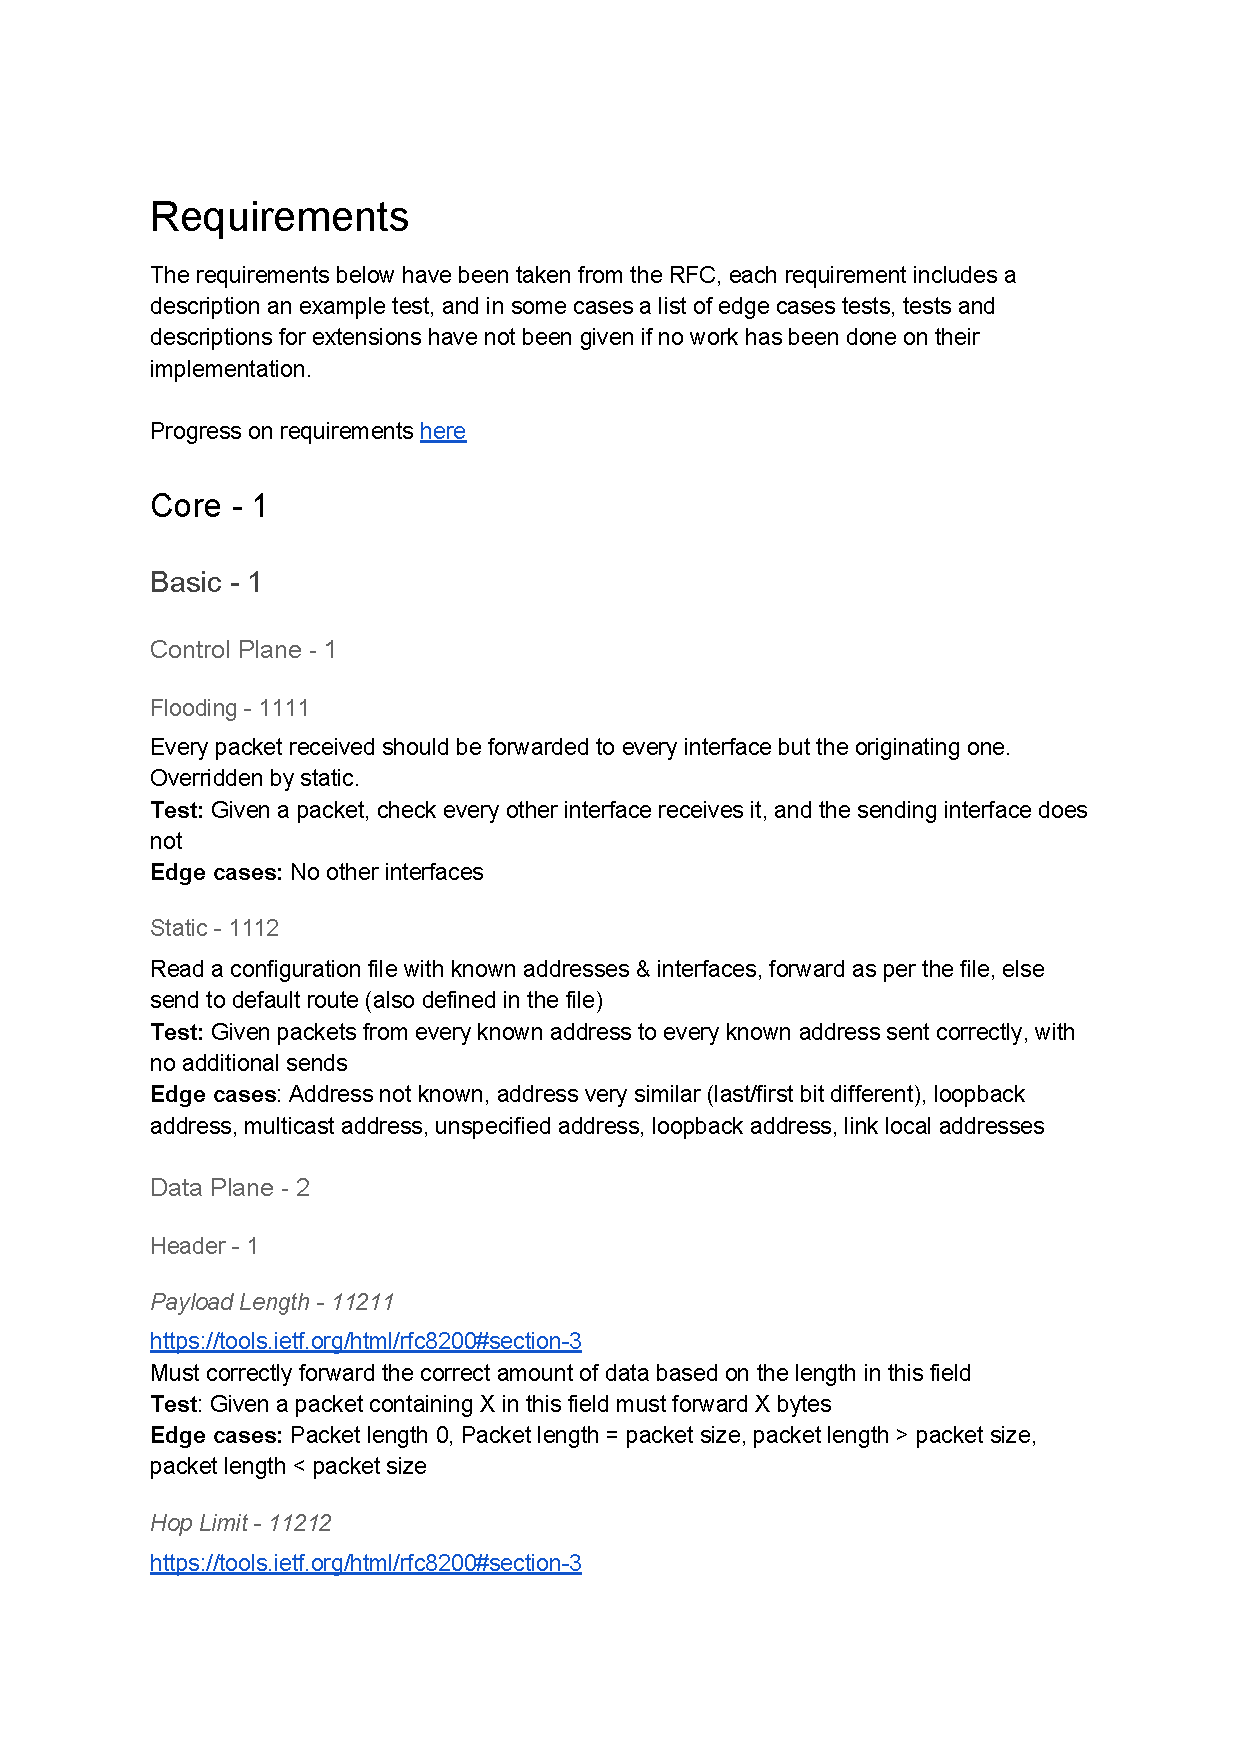
\includepdf[page=-]{requirements}


\chapter*{Project Proposal}
\addcontentsline{toc}{chapter}{Project Proposal}

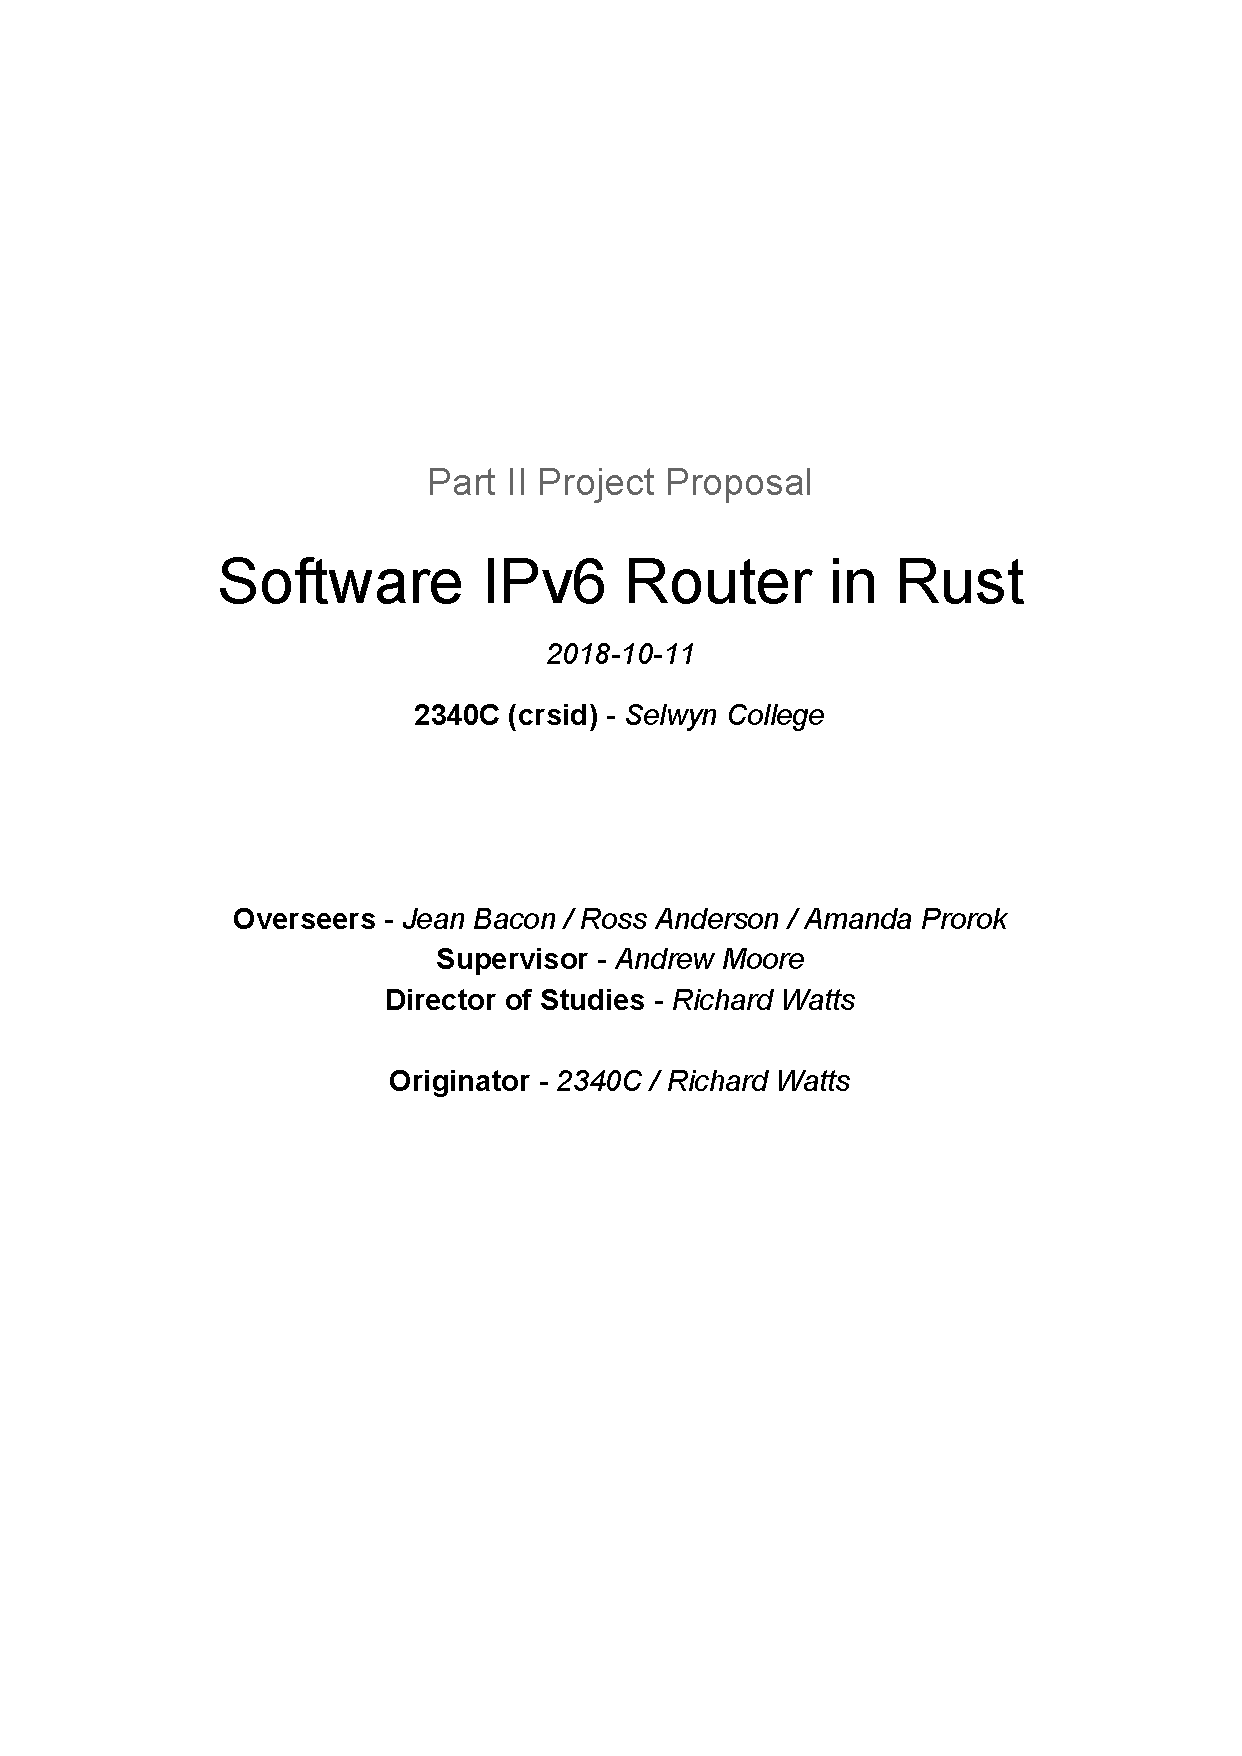
\includepdf[page=-]{proposal}

\end{document}